\section{Edge Detection}

What is an edge? An edge is contrast. We can visualise this by calculating the sobel edge magnitude and thresholded magnitude of an image.

\subsection{Differencing}

Horizontal differencing detects vertical edges, and vertical differencing detects horizontal edges. We can perform first order edge detection by adding the horizontal and vertical edges. This can be described mathematically as shown:

\begin{align}
    Evert_{x,y} = | P_{x,y} - P_{x+1,y} | \\[0.25cm]
    Ehrzn_{x,y} = | P_{x,y} - P_{x,y+1} | \\[0.25cm]
    E_{x,y} = | 2\times P_{x,y} - P_{x+1,y} - P_{x,y+1}|
\end{align}

We can use the coefficients of this equation to form the following template. However it is unnecessarily complex for this use.

\begin{equation}
    T = \begin{bmatrix}
            2 & -1 \\
            -1 & 0
        \end{bmatrix}
\end{equation}

\subsubsection{Uniform Thresholding}
We can select the brightest edge points using uniform thresholding. We select a threshold level to control the number of points.

\subsection{Analysis of Basic Operators}
Taylor series analysis reveals that differencing the adjancent points provides an estimate of the first order derivative at a point.
\\
If we separate points by $\Delta x$, then by the taylor expansion for $f(x+\Delta x$ is given by:

\begin{align}
   f(x+\Delta x) =  f(x) + \Delta x + f'(x) + \frac{\Delta x^{2}}{2!}\times f''(x) + \mathbf{O}(\Delta x^{3}) \\
   f'(x) = \frac{f(x+\Delta x) - f(x)}{\Delta x} - \mathbf{O}(\Delta x)
\end{align}

The difference between two adjacent points is an estimate of the first order derivative with an error of $O(\Delta x)$
The error is large when the interval size is large. The error is large if the curve is complex.

\textbf{Close sampling} is required for adequate approximation. We can reduce the error by spacing the differenced points by one pixel. This equivalent to computing the first order difference at two adjacent points as a new horizontal difference \textbf{Exx}.

\begin{equation}
    \textbf{Exx}_{x,y} = | P_{x+1,y} + P_{x-1,y} |
\end{equation}

We can analyse this by taylor series and expand $f(x-\Delta x)$. We obtain the first order derivative through rearranging as:

\begin{equation}
    f'(x) = \frac{f(x+\Delta x) - f(x-\Delta x)}{2\Delta x} - \mathbf{O}(\Delta x^{2})
\end{equation}

The error is now $O(\Delta x^{2})$ Leaving us with the templates for horizontal and vertical first order difference.

\begin{align}
    \text{Mx }\begin{bmatrix}
    1 & 0 & -1
    \end{bmatrix} \\ 
    \text{My }\begin{bmatrix}
    1 \\
    0 \\
    -1
    \end{bmatrix}
\end{align}

\subsection{Prewitt Operator}
Edge detection is similar to differentiation, as it detects change, it is also bound to noise. Therefore we should also apply averaging to reduce noise with the detection process.

Which leaves us with the following templates. By extending Mx and My for the horizontal and vertical templates.

\begin{table}[h!]
    \centering
    \begin{tabular}{cc}
       \begin{bmatrix} 1 & 0 & -1 \\ 1 & 0 & -1 \\ 1 & 0 & -1 \end{bmatrix}  & \begin{bmatrix}
           1 & 1 & 1 \\ 0 & 0 & 0 \\ -1 & -1 & -1
       \end{bmatrix} \\
    \end{tabular}
    \caption{Templates for Prewitt Operator}
    \label{tab:prewitt}
\end{table}

This returns the rate of change of brightness along each axis. The edge magnitude, and edge direction.

\begin{align}
    M(x,y) = \sqrt{Mx(x,y)^{2} + My(x,y)^{2}} \\
    \theta(x,y) = \arctan(\frac{My(x,y)}{Mx(x,y)})
\end{align}

\subsubsection{Implementation}

When applied to the image of a square, we obtain the edge magnitude and direction.

\begin{figure}[!h]
    \centering
    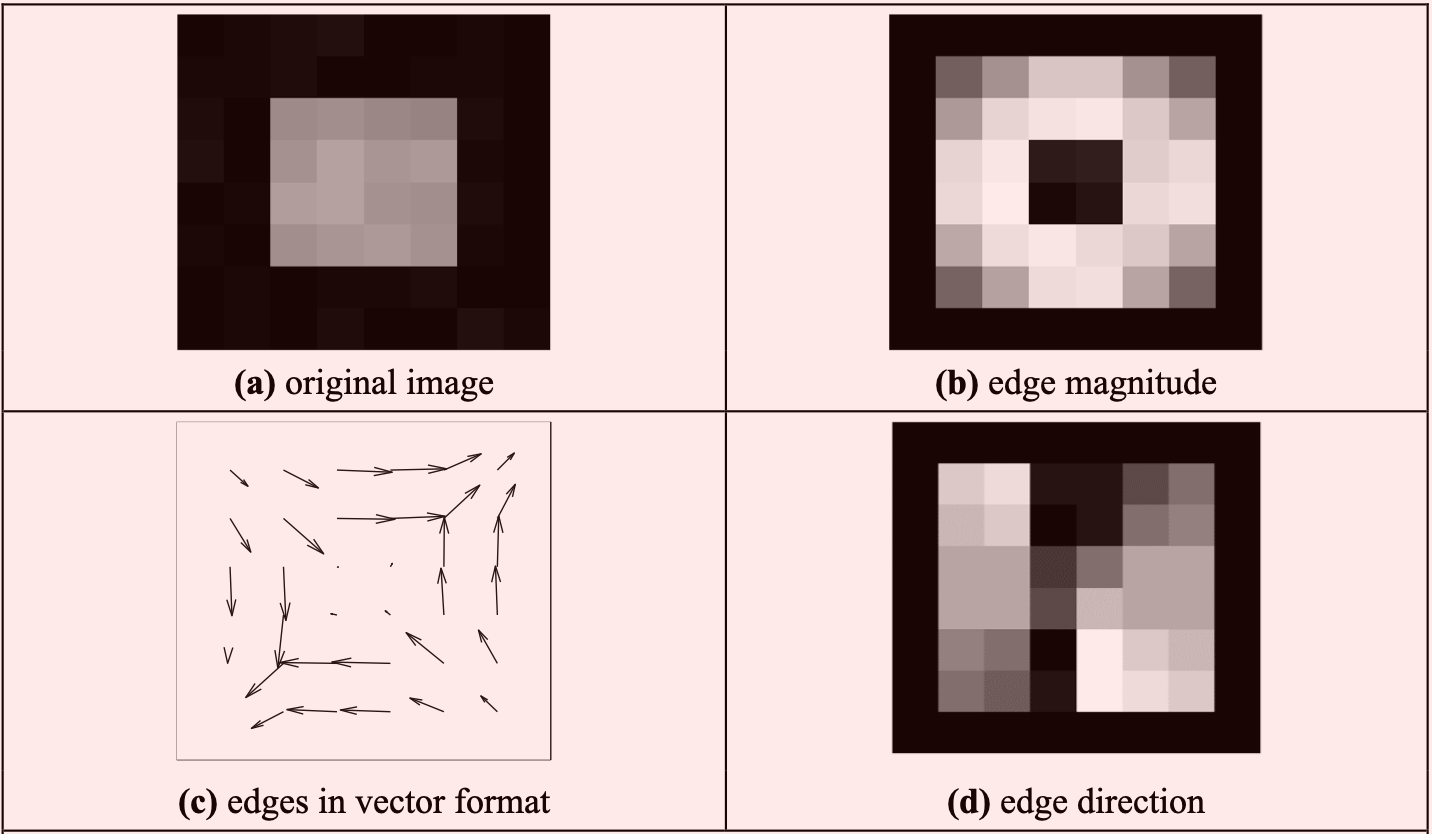
\includegraphics[scale=0.4]{Images/Prewitt.png}
    \caption{Applied Prewitt Operator}
    \label{fig:prew}
\end{figure}

Template convolution could be applied here, but it is not necessary.

\subsection{Sobel Edge Detection}
When the weight at the central pixels for both Prewitt templates is doubled, two templates for the Sovel edge detection are formed.

\begin{table}[h!]
    \centering
    \begin{tabular}{cc}
       \begin{bmatrix} 1 & 0 & -1 \\ 2 & 0 & -2 \\ 1 & 0 & -1 \end{bmatrix}  & \begin{bmatrix}
           1 & 2 & 1 \\ 0 & 0 & 0 \\ -1 & -2 & -1
       \end{bmatrix} \\
    \end{tabular}
    \caption{Templates for Prewitt Operator}
    \label{tab:sobel}
\end{table}

The implementation is similar, however we can use larger templates to introduce more smoothing, noise reduction, but edge blurring becomes a problem. \\

Given that \textbf{Gaussian averaging produces optimal averaging}, we can use the binomial expansion to approximate the gaussian normal distribution. It is essential a gaussian operator with integer coefficients. To generalise sobel, we use the differencing coefficients in a binomial expansion.

\subsubsection{Evaluation of Sobel}
\begin{itemize}
    \itemsep0em
    \item Sobel is a good basic operator
    \item - Blurred edges
    \item - Noisy edges
\end{itemize}

\subsection{Canny Edge Detection}

Canny gives thin edges in the correct place but it is more complex.

The general process for canny edge detection is as follows:

\begin{itemize}
    \item [1] Gaussian smoothing to reduce noise
    \item [2] Sobel edge detection
    \item [3] Reduce blurred edges and noise through non maximum suppresion
    \item [4] Hysteresis thresholding to connect edge points
\end{itemize}

\subsubsection{Operator}
Objectives of the Canny Edge Detector
\begin{itemize}
    \itemsep0em 
    \item Optimal detection without spurious responses
    \item Good localisation with minimal distance between edge detected and the true edge.
    \item Single response to eliminate multiple responses to a single edge.
\end{itemize}

We 'walk' along the top of the edge, to give thin edges in the right place.

\subsubsection{Interpolation in non-maximum Suppression}
Need to use points which are not on the image grid, we can do this through linear interpolation.

\subsubsection{Hysteresis Thresholding Transfer Function}
Lower threshold = average noise \\
Upper threshold = average feature boundary.

\subsection{Comparisons}

Hysteresis thresholding gives all points $>$ upper threshold, plus any connected points $>$ lower threshold.
\\
We get less noise, and better \textit{thinner} edges.

\subsection{Edge Detection via Laplacian Operator}

We can describe the second order (laplaian of gaussian) edge detection process mathematically as follows:

\begin{align}
    g(x,y,\sigma) = e^{\frac{-(x^{2}+y^{2)}}{2\sigma^{2}}} \\
    \frac{\delta g(x,y,\sigma)}{\delta x} = -\frac{x}{\sigma^{2}} e^{\frac{-(x^{2}+y^{2)}}{2\sigma^{2}}} \\
    \frac{\delta^{2}g(x,y,\sigma)}{\delta^{2}x^{2}} = (\frac{x^{2}}{\sigma^{2}}-1)\frac{e^{\frac{-(x^{2}+y^{2)}}{2\sigma^{2}}}}{\sigma^{2}} \\
    \text{Given that: }\nabla^{2}g(x,y,\sigma) = \frac{\delta^{2}g(x,y,\sigma)}{\delta^{2}x^{2}}U_{x} + \frac{\delta^{2}g(x,y,\sigma)}{\delta^{2}y^{2}}U_{y} \\
    = (\frac{x^{2}}{\sigma^{2}}-1)\frac{e^{\frac{-(x^{2}+y^{2)}}{2\sigma^{2}}}}{\sigma^{2}} + (\frac{y^{2}}{\sigma^{2}}-1)\frac{e^{\frac{-(x^{2}+y^{2)}}{2\sigma^{2}}}}{\sigma^{2}} \\
    \nabla^{2}g(x,y,\sigma) = \frac{1}{\sigma^{2}}(\frac{x^{2}+y^{2}}{\sigma^{2}}-2)\times\e^{\frac{-(x^{2}+y^{2)}}{2\sigma^{2}}}
\end{align}

\subsection{Zero crossing detection}
Need to find zero-crossings in 2D.
\begin{equation}
    IF(max(1,2,3,4)>0\Andmin(1,2,3,4)<0) {f(x,y) = edge}
\end{equation}

\subsection{Marr-Hildreth Edge Detection}

Given the second order laplacian of gaussian edge detection, we can detect local features with a small template. We use a larger template to detect global features.